\documentclass{article}

\usepackage[utf8]{inputenc}
\usepackage[T1]{fontenc}      
\usepackage[francais]{babel}
\usepackage{graphicx}
\usepackage{circuitikz}
\usepackage[squaren, Gray]{SIunits}
\usepackage{sistyle}
\usepackage[autolanguage]{numprint}
\usepackage{pgfplots}
\usepackage{amsmath,amssymb,array}
\usepackage{url} 

% New command pour la modélisation mécanique, tri à effectuer
\newcommand\fv[1]{{\bf #1}} % free vector
\newcommand\fvd[1]{\dot{\bf #1}} % free vector derivated
\newcommand\fvdd[1]{\ddot{\bf #1}} % free vector derivated
\newcommand\fvr[1]{\mathring{\bf #1}} % free vector relatively derivated
\newcommand\fvrr[1]{\overset{\circ\circ}{\bf #1}} % free vector relatively derivated
\newcommand\uv[1]{{\bf\hat{ #1}}} % unit vector
\newcommand\ui{{\bf\hat{I}}} % unit vector I
\newcommand\uj{{\bf\hat{J}}} % unit vector J
\newcommand\uk{{\bf\hat{K}}} % unit vector K
\newcommand\wrt[2]{\ensuremath{\tensor*[_{ #1}]{ #2}{}}} % With Respect To
\newcommand\wtr[3]{\ensuremath{\tensor*[_{ #1}]{ #2}{^{ #3}}}} % With Two Respect
\newcommand\omegaf{{\bm \omega}}
\newcommand\omegafr{\mathring{\bm \omega}}
\newcommand\omegafd{\dot{\bm \omega}}
\newcommand\omegaft{\tilde{\bm \omega}}
\newcommand\omegaftr{\mathring{\tilde{\bm \omega}}}
\newcommand\omegat{\tilde{\omega}}
\newcommand\omegatd{\tilde{\dot{\omega}}}
\newcommand\ine{{\bf I}}
\newcommand\st{{\bf L}}
\newcommand\pst{{\bf M}}
\newcommand\lm{{\bf N}}
\newcommand\am{{\bf H}}
\newcommand\amd{\dot{\am}}
\newcommand\fo{{\bf F}}
\newcommand\po{\mathcal{P}}
\newcommand\xg{\ensuremath{\fv{R}}}
\newcommand\xgd{\ensuremath{\fvd{R}}}
\newcommand\xgdd{\ensuremath{\fvdd{R}}}
\newcommand\dvec[1]{\dot{\vec{ #1}}}
\newcommand\ddvec[1]{\ddot{\vec{ #1}}}
\newcommand\qp{\dot{q}}
\newcommand\dqp{\Delta \dot{q}}

\begin{document}

Voici quelques traces de nos  mesures en laboratoire:


\begin{figure}[ht!]
    \centering
    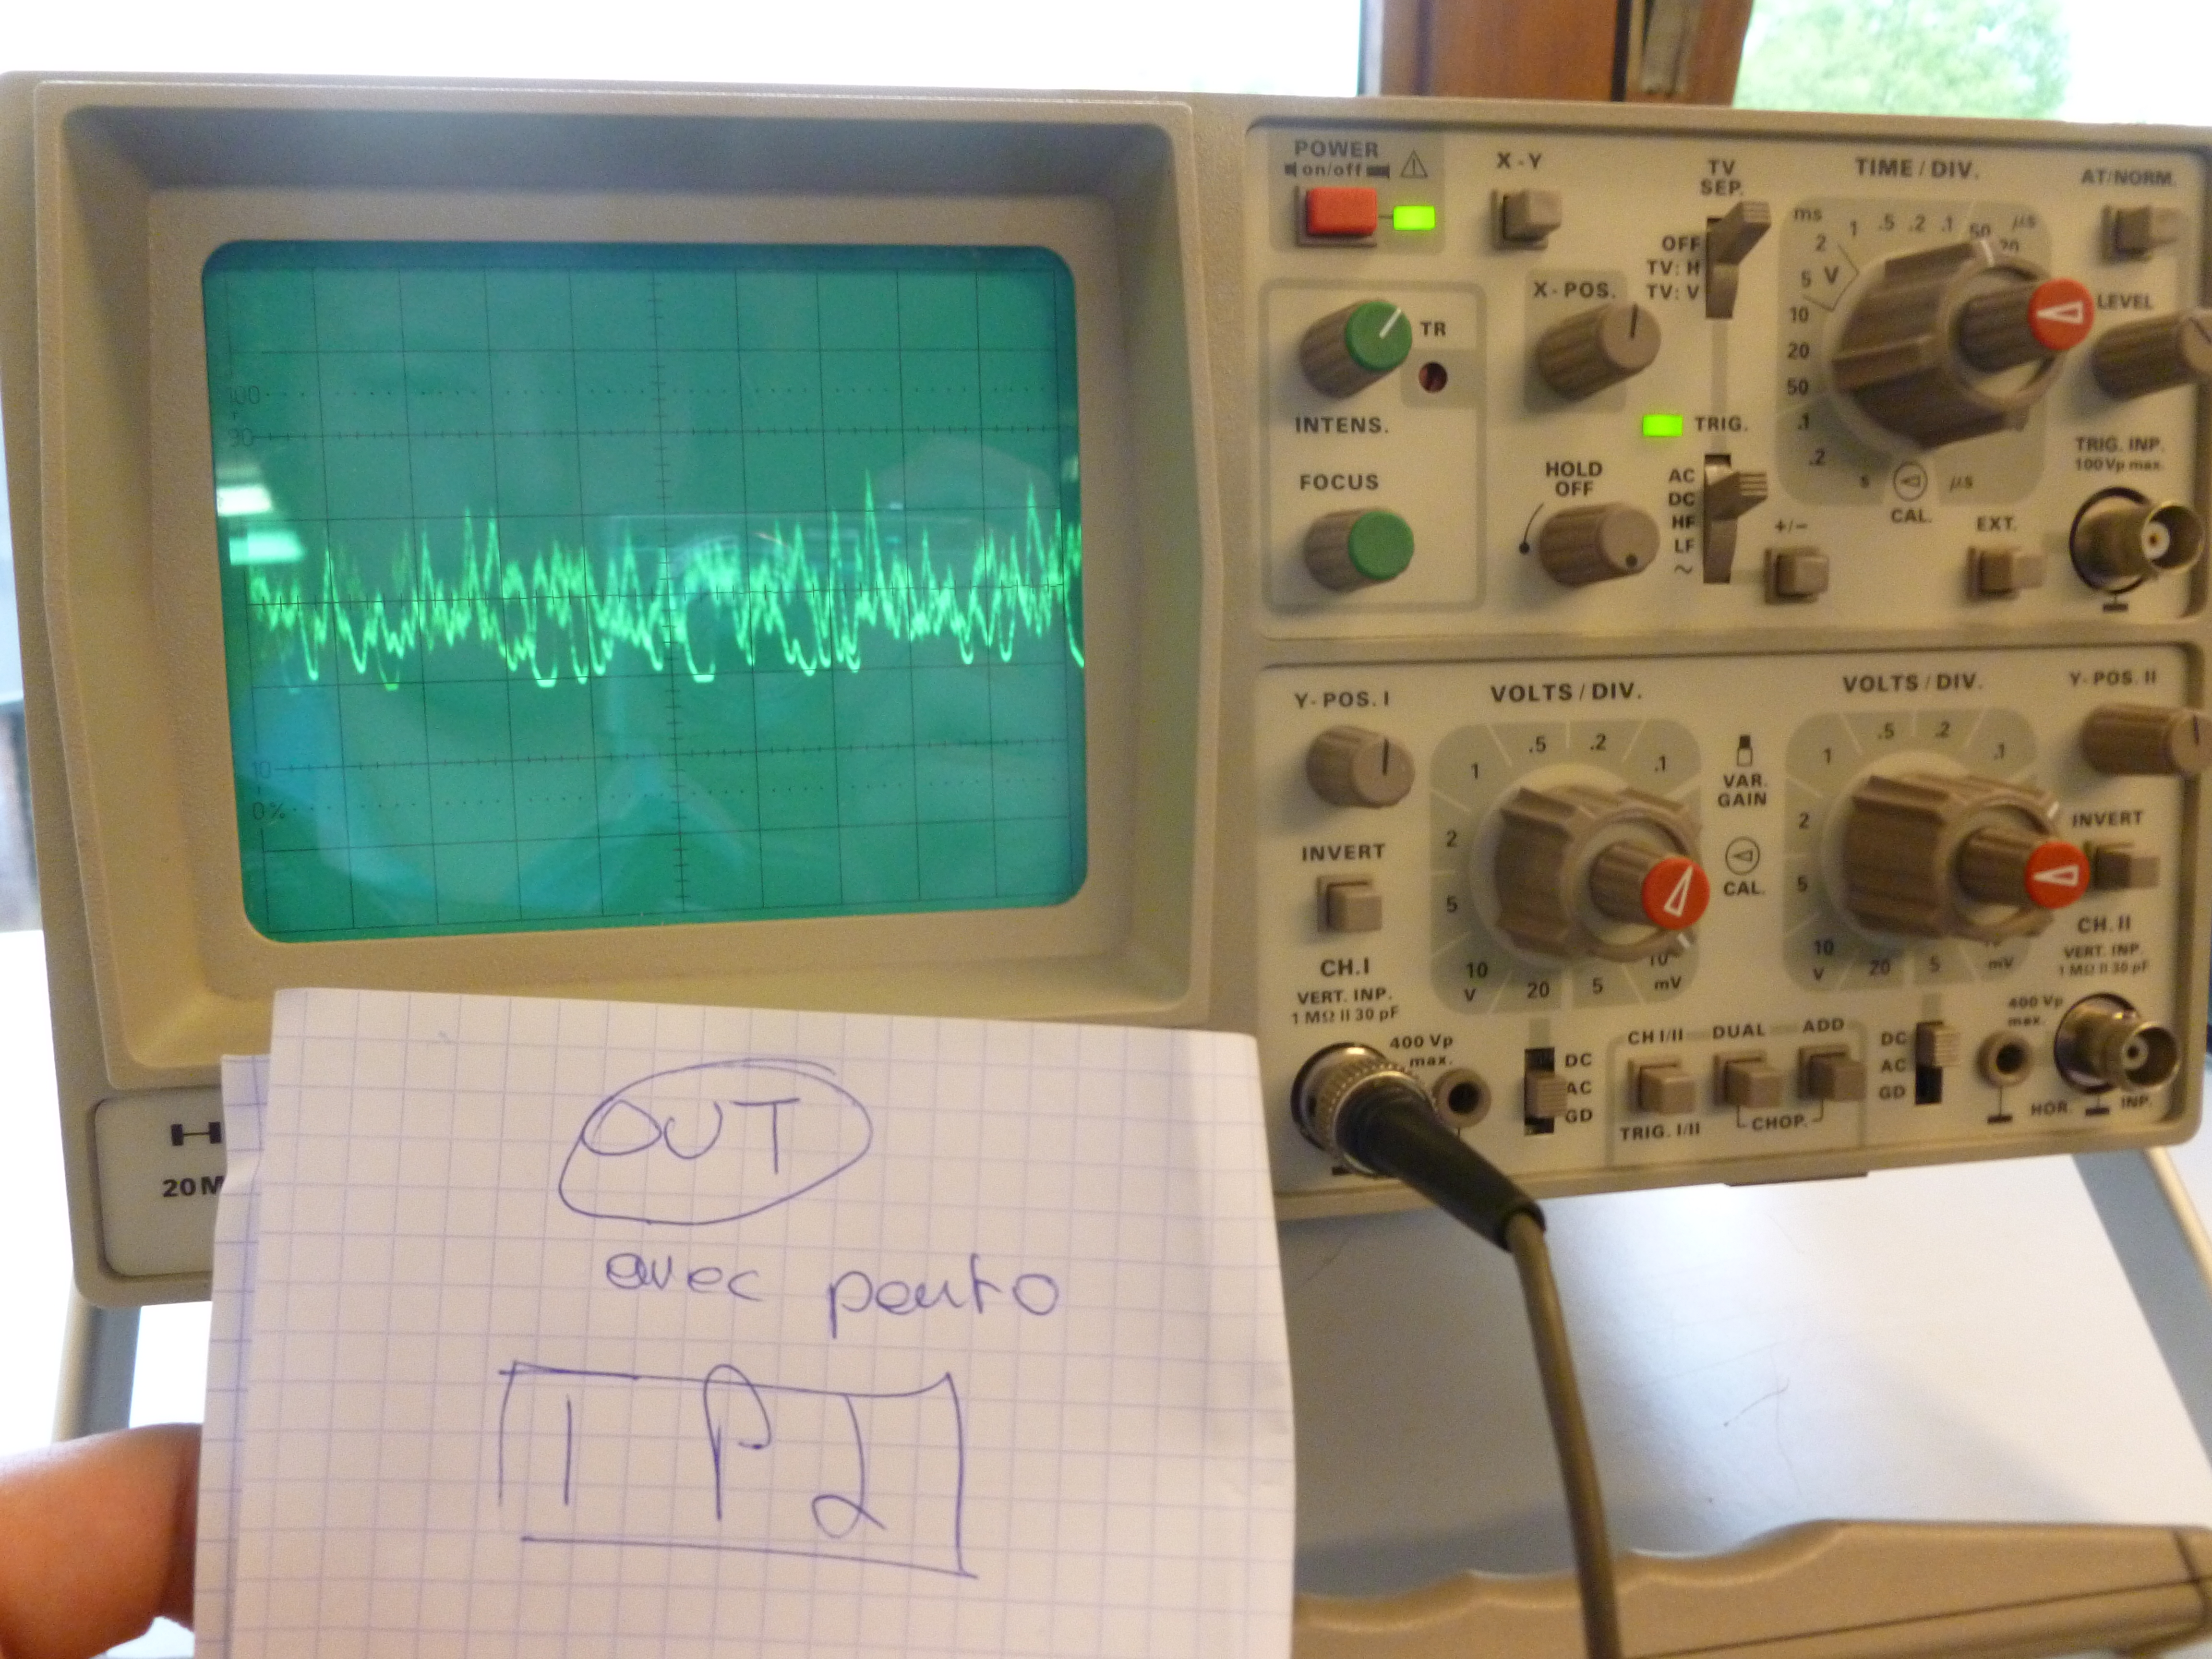
\includegraphics[scale=0.05]{P1010038.jpg}
    \caption{TP2}
    \label{TP2}
\end{figure}

\begin{figure}[ht!]
    \centering
    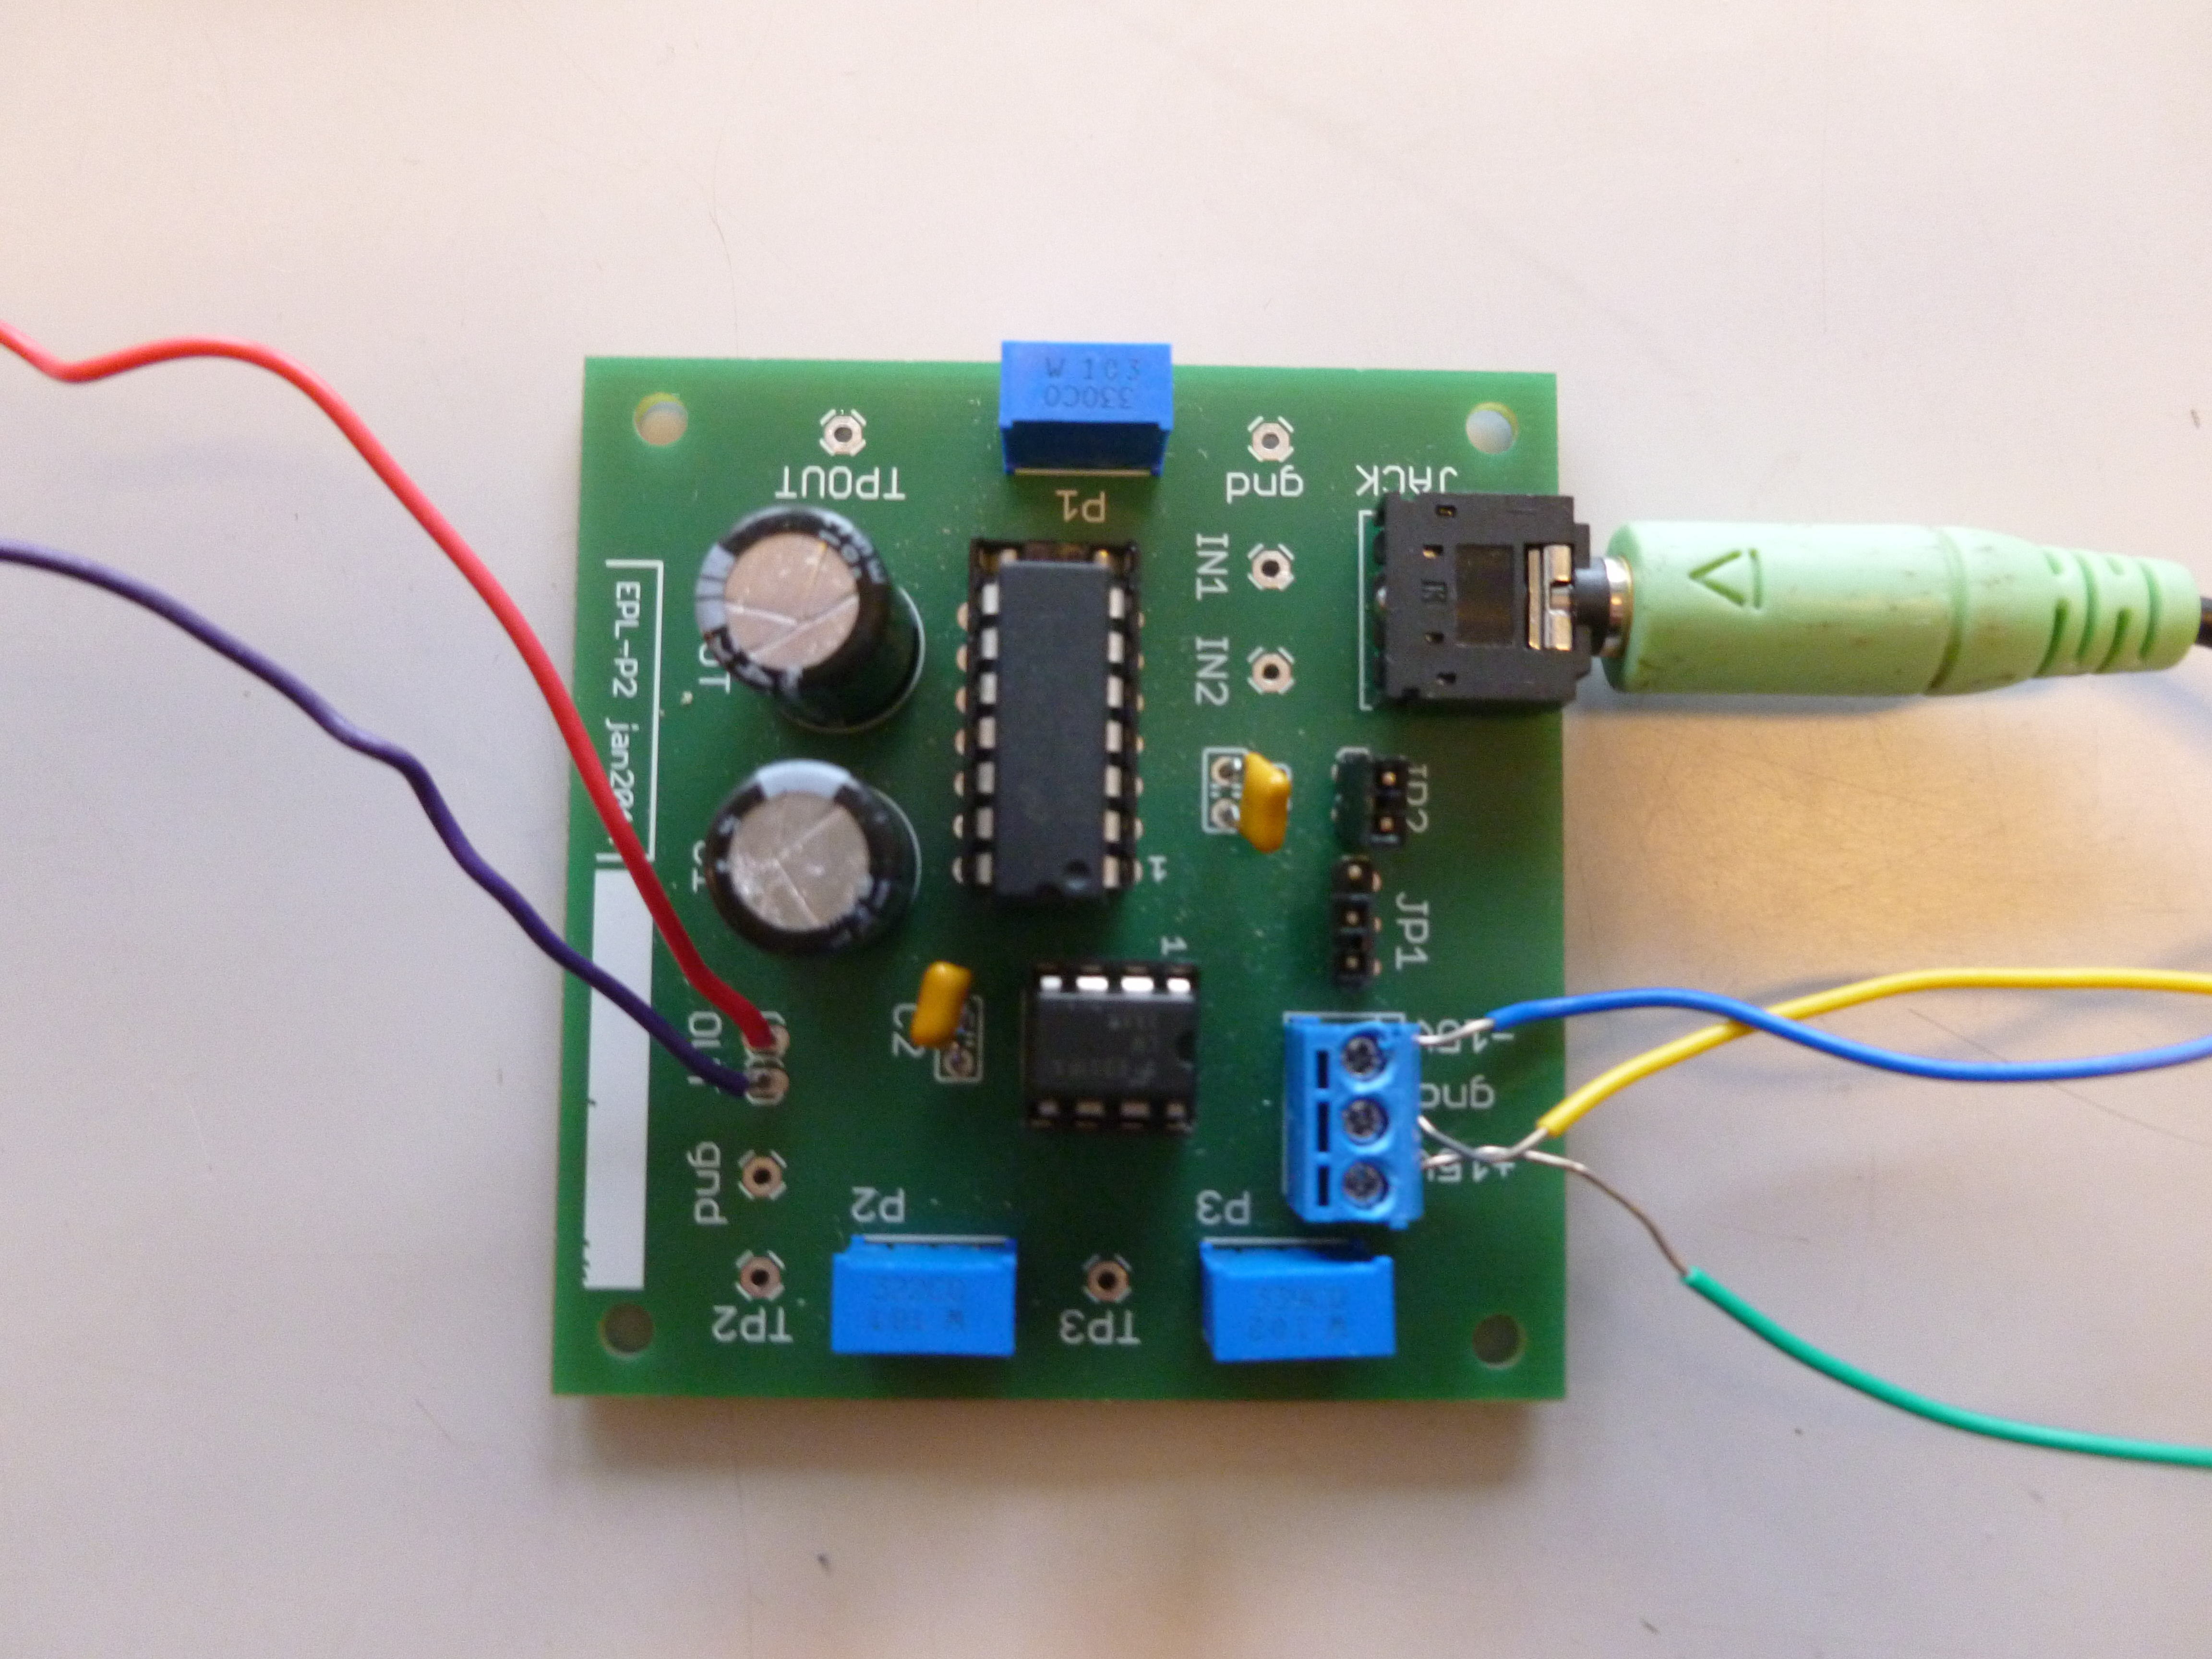
\includegraphics[scale=0.05]{P1010039.jpg}
    \caption{Schéma de la plaquette}
    \label{plaquette}
\end{figure}

\begin{figure}[ht!]
    \centering
    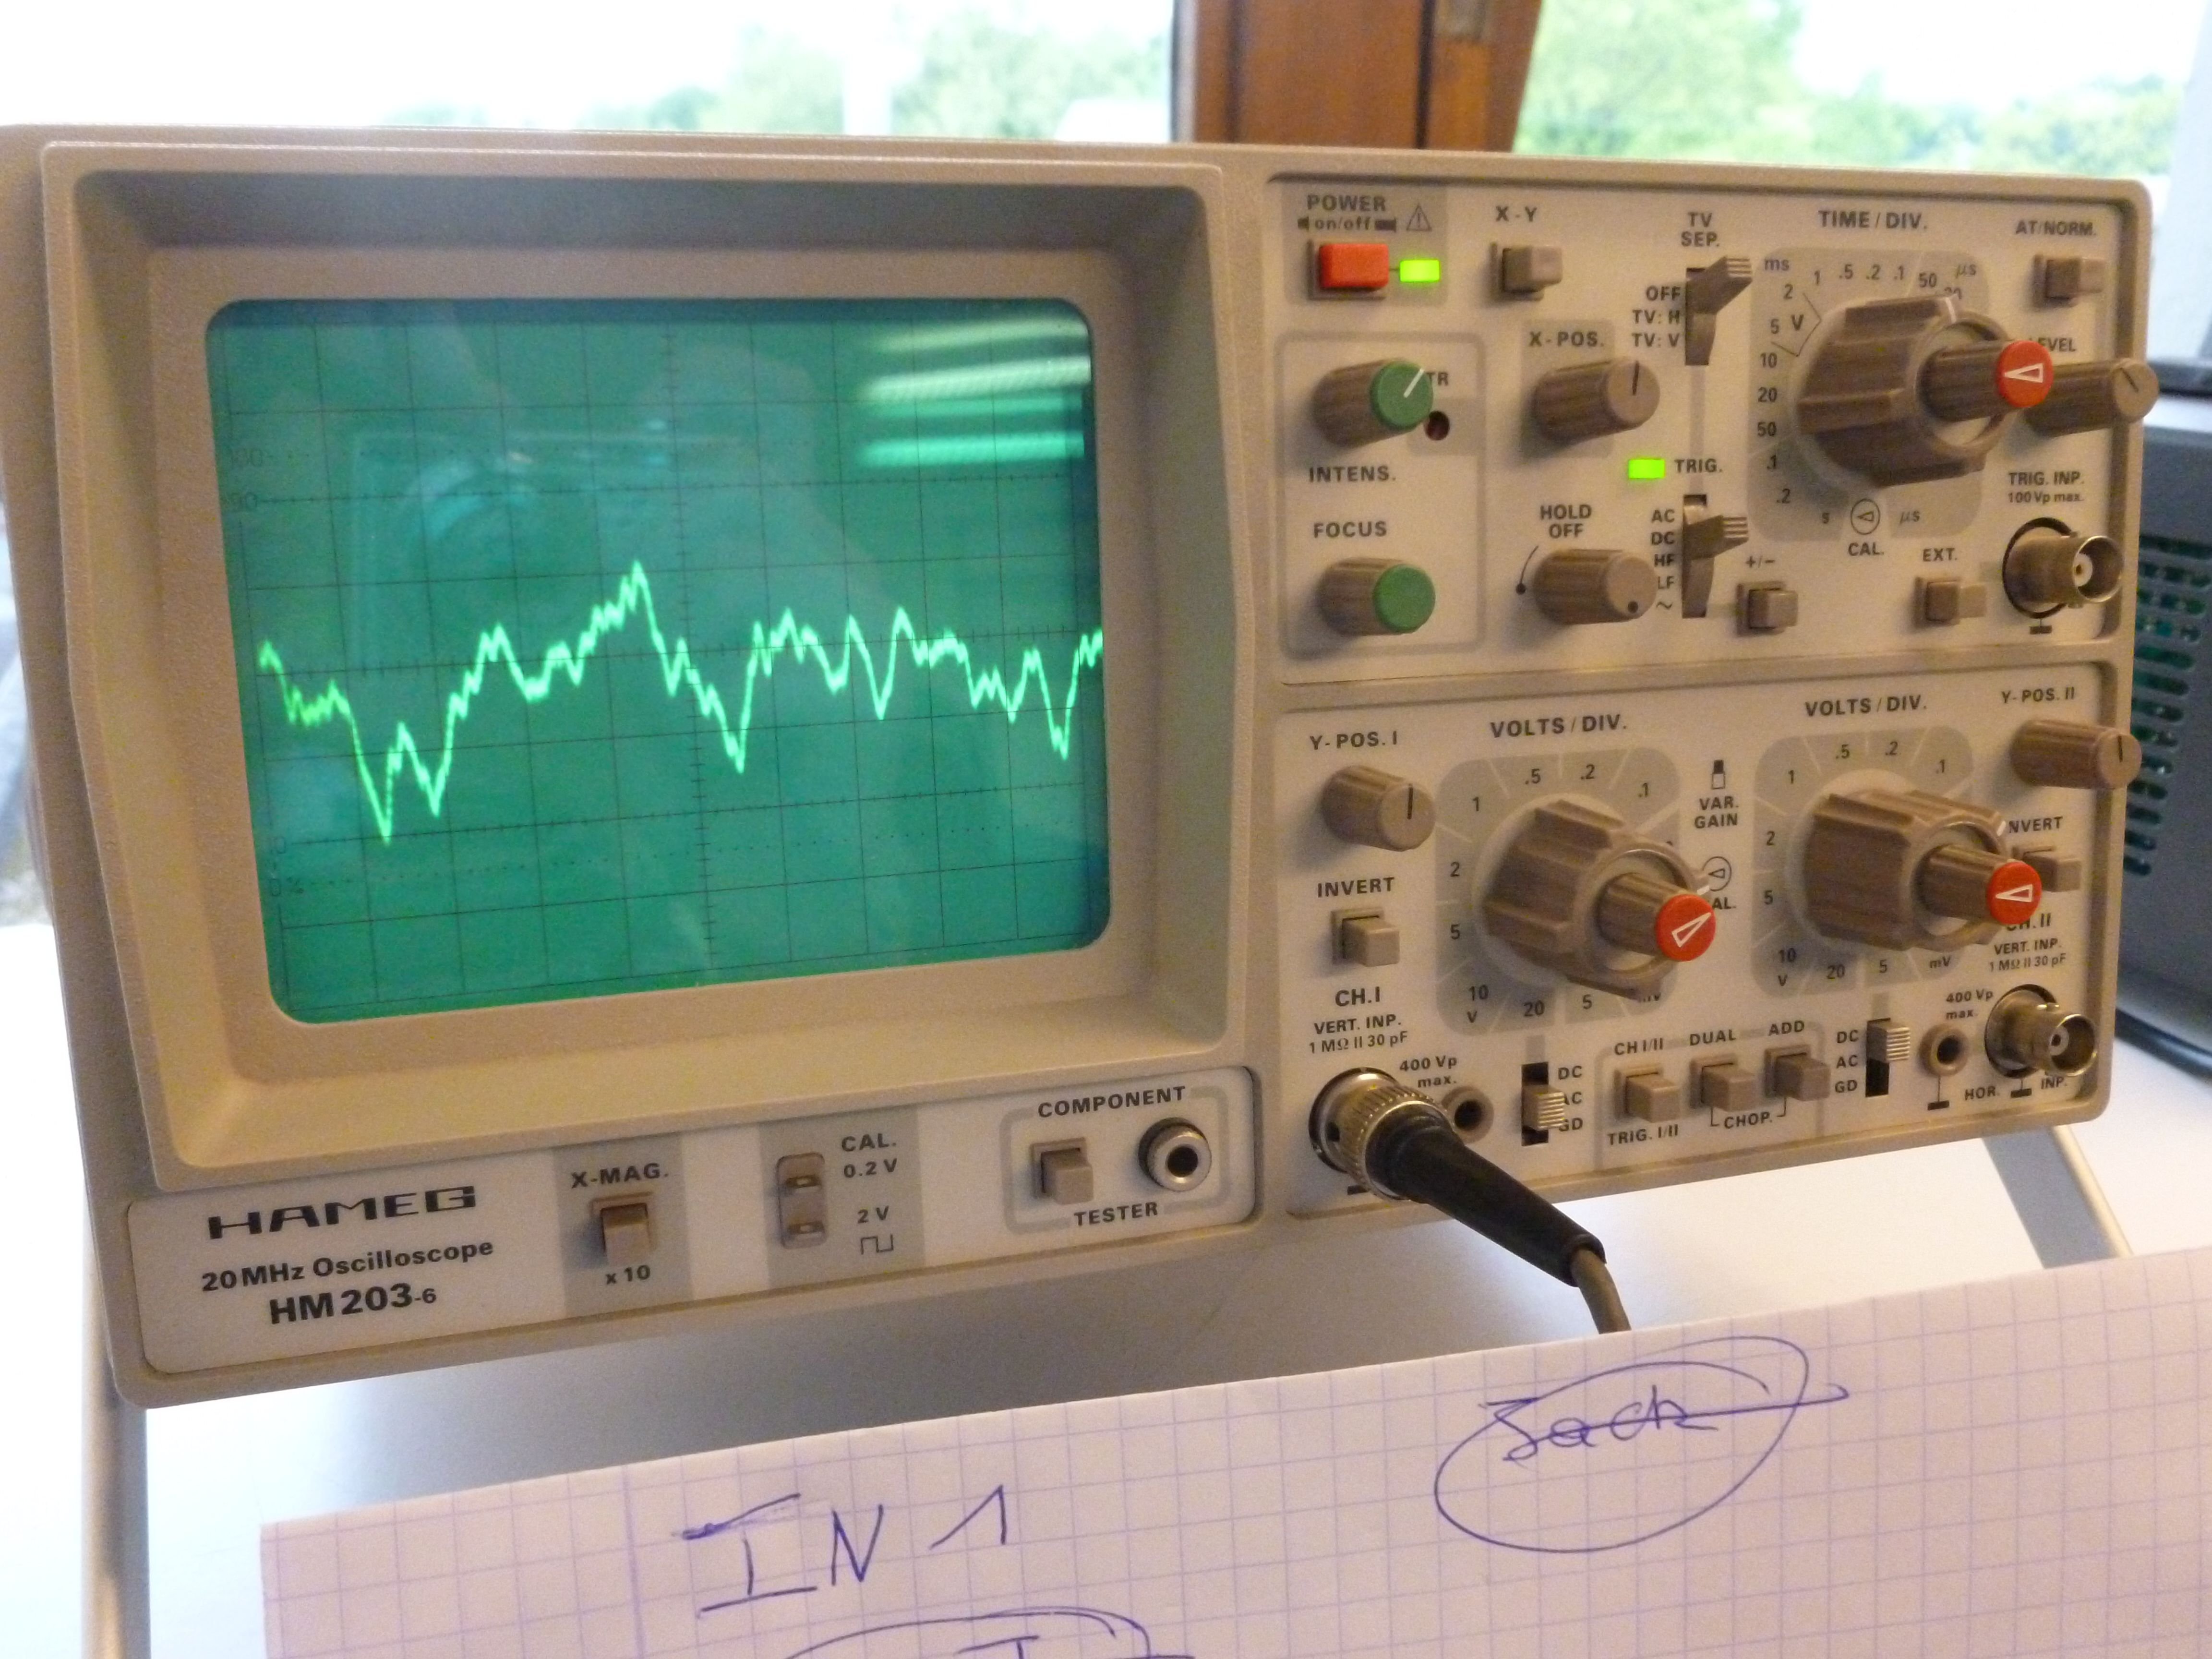
\includegraphics[scale=0.05]{P1010034.jpg}
    \caption{IN1}
    \label{IN1}
\end{figure}

\begin{figure}[ht!]
    \centering
    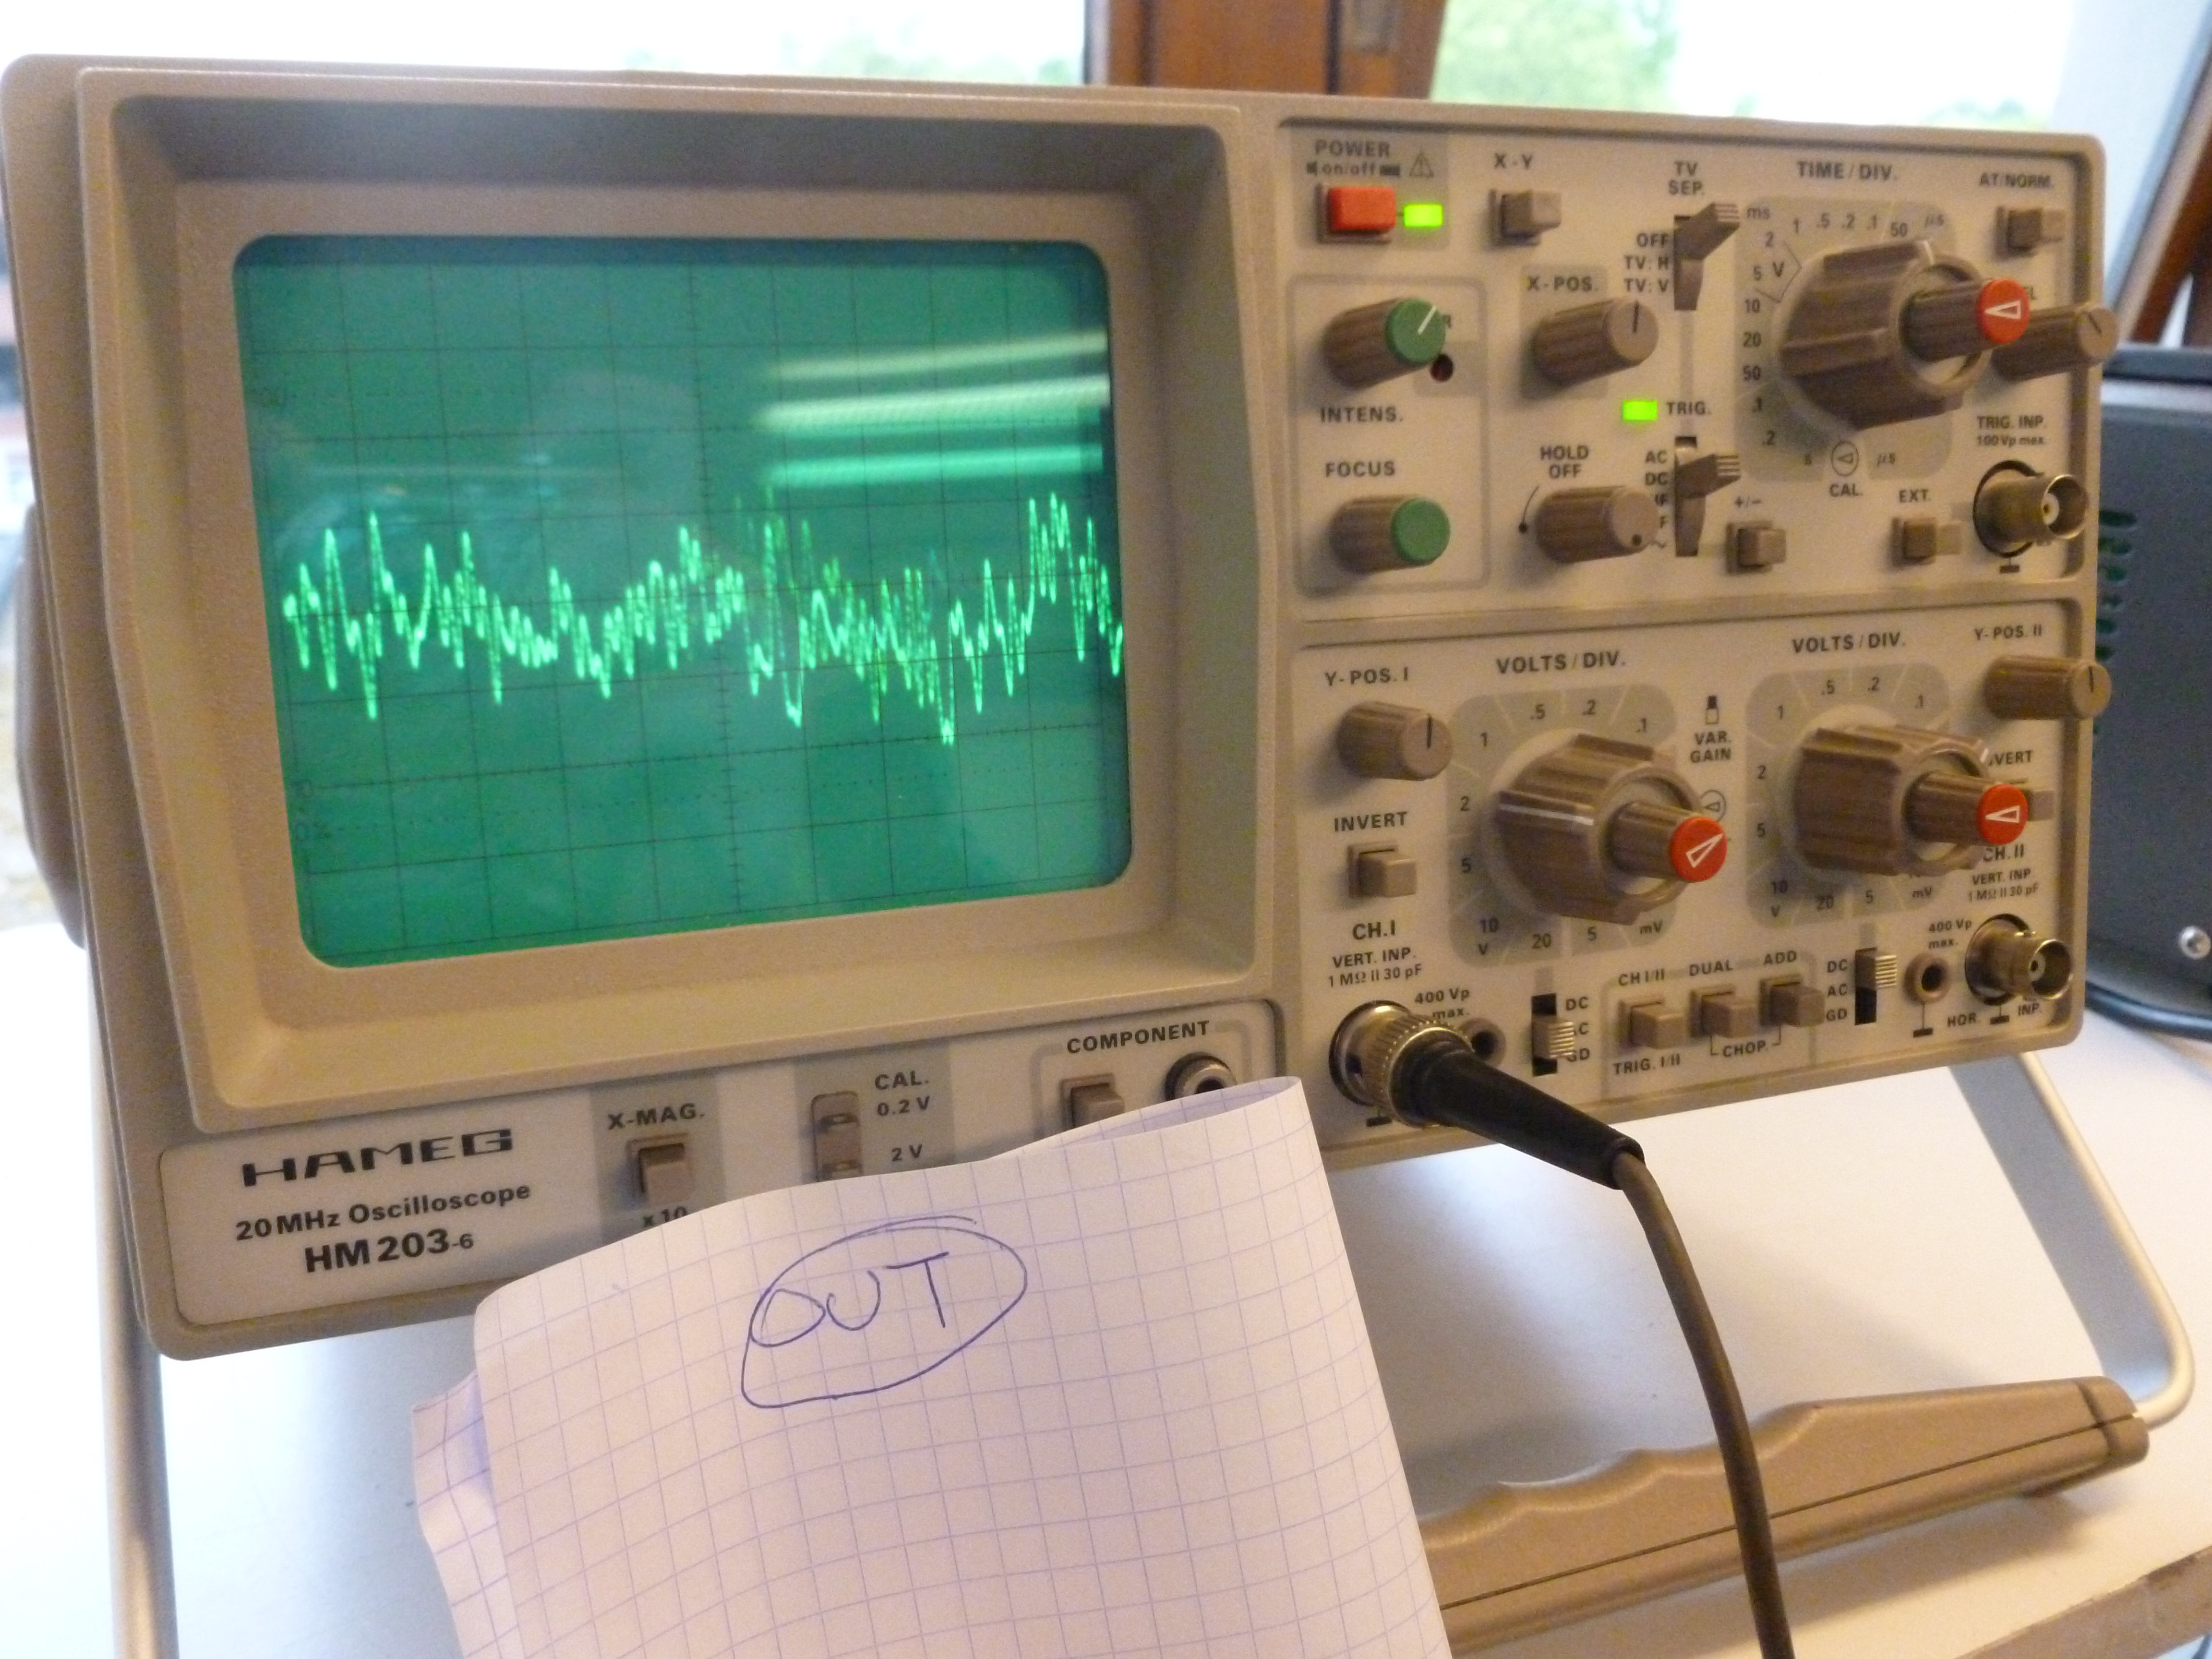
\includegraphics[scale=0.05]{P1010035.jpg}
    \caption{OUT}
    \label{OUT}
\end{figure}

% Just here to fix rapport_prejury.tex
\end{document}
